\documentclass[colorlinks]{article}
\usepackage{graphicx}

\usepackage{hyperref,verbatim}
\usepackage[usenames, dvipsnames]{color}
\usepackage{tgpagella} % text only
\usepackage{mathpazo} 
\usepackage[margin=0.6in]{geometry}
\addtolength{\topmargin}{0in}


\newcommand{\deadline}{Noon Jan 15}
\newcommand{\extdeadline}{Noon Jan 16}
\newcommand{\total}{25}

%opening
\title{Machine Learning\\Homework 1 : Decision Trees and Ensemble Methods\\(due \deadline)}
\author{}
\date{}

\begin{document}

\maketitle

\noindent\fbox{
	\parbox{\textwidth}{
		Instructions\\
		\begin{enumerate}
			\item In case you are unfamiliar with the Python data ecosystem (NumPy, Pandas), you are recommended to study the first four chapters of the \href{https://jakevdp.github.io/PythonDataScienceHandbook/}{Python data science handbook}. A doubt clearing session would be organised in case you have any difficulties in the data science ecosystem.
			\item The deadline for full score is \deadline. You can get 50\% credit for late submission (\extdeadline).
			\item Total marks = \total
			\item You have to type the assignment using a word processing engine, create a pdf and upload on the form. Please note that only pdf files will be accepted.
			\item All code/Jupyter notebooks must be put up as \href{https://gist.github.com/}{\textbf{secret gists}} and linked in the created pdf submission. Again, only secret gists. Not public ones.
			\item Any instances of cheating/plagiarism will not be tolerated at all. 
			\item Cite all the pertinent references in IEEE format.
			\item The least count of grading would be 0.5 marks. 

		\end{enumerate}
	}
}

\begin{figure}
	\centering
	\vspace{-100pt}
	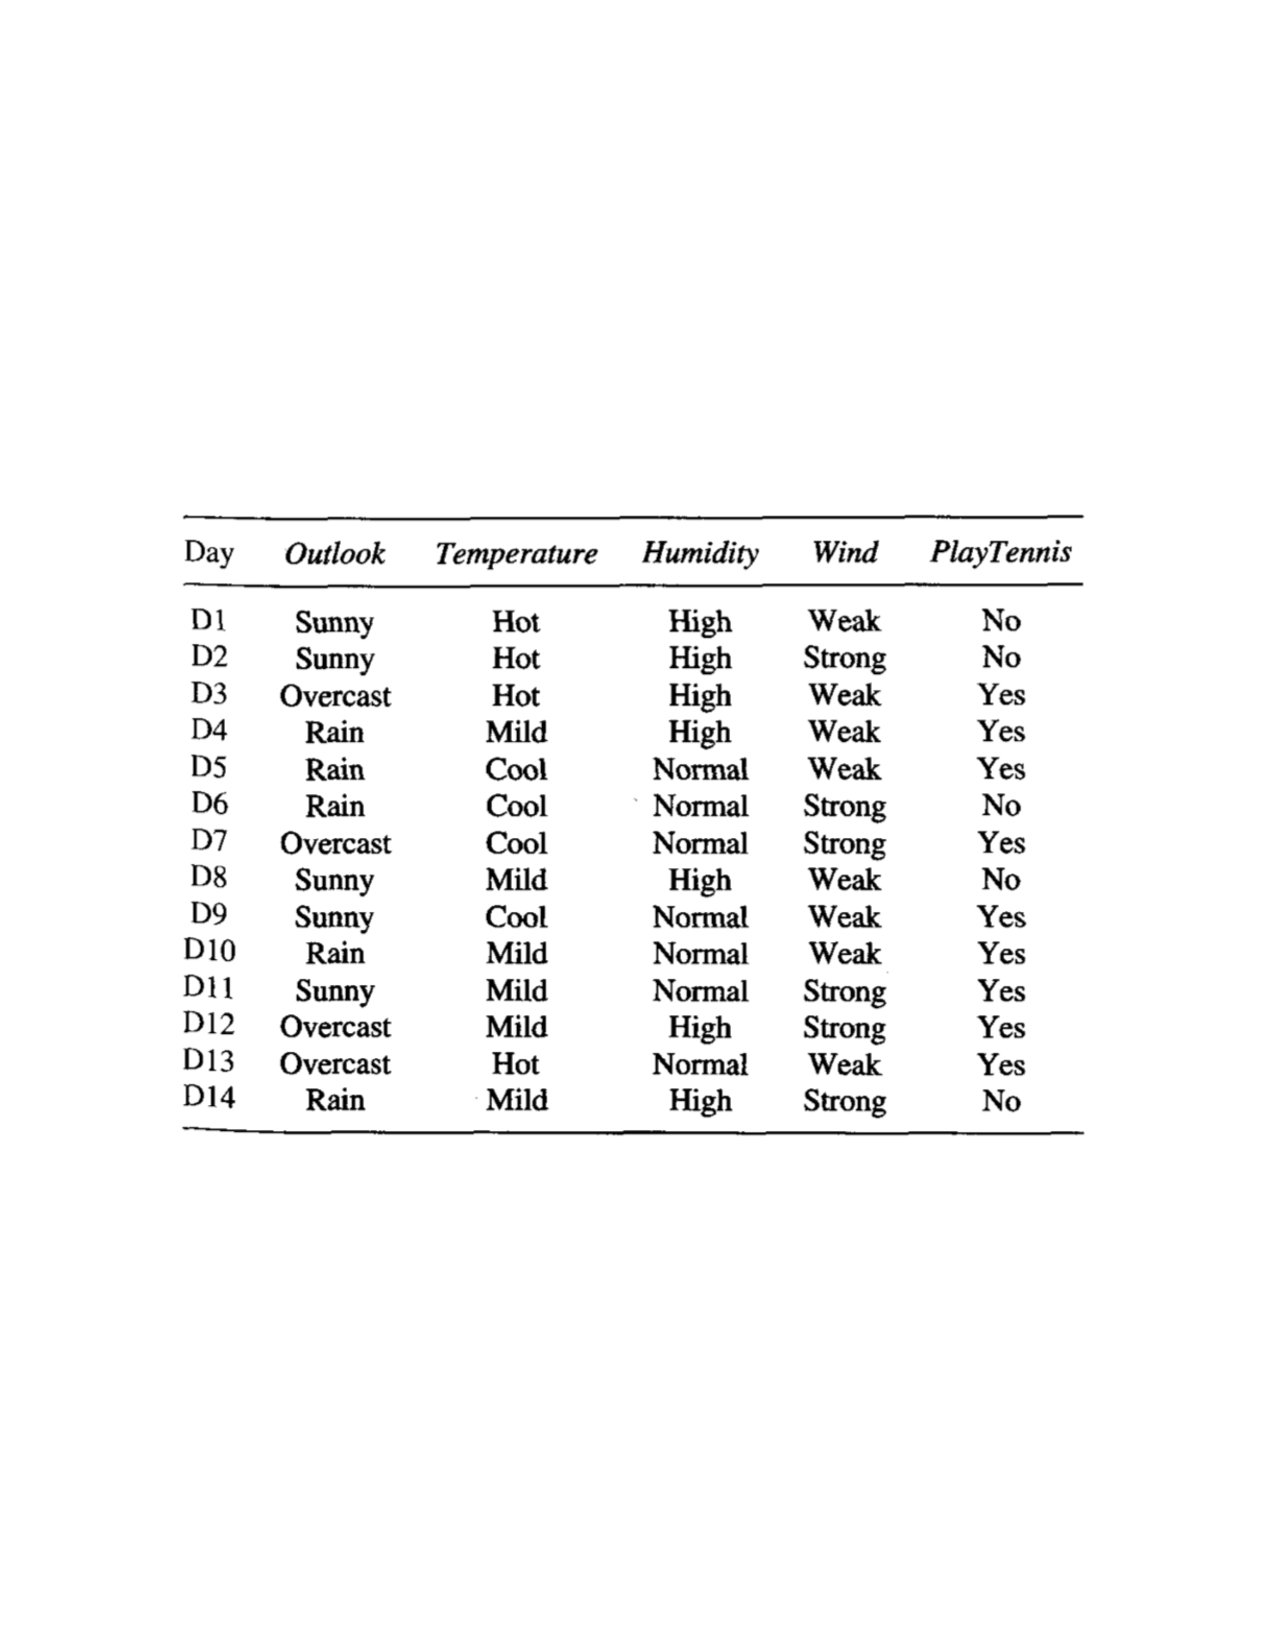
\includegraphics[scale=0.5]{dt-dataset.pdf}
	\vspace{-100pt}
	\caption{PlayTennis Dataset}
	\label{fig:dt-dataset}
\end{figure}


\begin{enumerate}
	\item 	\begin{enumerate}
		\item For the following dataset shown in Figure~\ref{fig:dt-dataset}(~same as the one we used in the class), now let us assume that date is also an input feature. Which attribute will be chosen as the root node for the decision tree? Do you think choosing this attribute is a good choice? Explain your answer.  \textbf{[1 mark]}
		\item Handling missing values in decision trees: Assume that the Outlook of D3 is missing. Could you still learn a decision tree from this example. The set of features of interest are: Outlook, Temperature, Humidity and Wind. Clarifiying again - Day is \textbf{not} to be used as a feature in this sub part of the question. Refer to Tom Mitchell Chapter 3.7.4 last paragraph and show the learnt decision tree despite the missing Outlook values from D3.  \textbf{[1 mark]}
	\end{enumerate}



\item 	\begin{enumerate}
	

	
		\item Write a Jupyter notebook to create a decision tree from scratch using the \href{https://www.stat.wisc.edu/~loh/treeprogs/guide/wires11.pdf}{CART algorithm}. The code should be written in native Python and not use existing libraries. The code should work for regression and classification tasks. As a hint: you may want to use dictionaries to encode the nested relationship amongst the different nodes, eg. tree = \`feature1' :\{`val1': ..., `val2', ...\}\}. \textbf{[4 marks]}
		\item Show the usage of your decision tree on the IRIS dataset. The first 70\% of the data should be used for training purposes and the remaining 30\% for test purposes. Show the accuracy of the decision tree you implemented on the test dataset. \textbf{[1 mark]}
		\item Use 5 fold cross-validation on the dataset. Using nested cross-validation find the optimum depth of the tree. \textbf{[2 marks]}
	\end{enumerate} 
	
	\item Show the usage of your decision tree for the \href{https://archive.ics.uci.edu/ml/datasets/Real+estate+valuation+data+set}{real estate price prediction regression} problem. \textbf{[1 mark]}
	\item Compare the performance of your model with the decision tree module from scikit learn. \textbf{[1 mark]}
	\item Use \href{https://github.com/parrt/dtreeviz}{dtreeviz} in conjunction with your library to show the learnt decision trees for the above two problems. What can you infer from this visualisation? \textbf{[2 marks]}
	\item For the IRIS dataset classification problem, consider three variants of the decision tree algorithm. In the best case, we do an exhaustive search over all possible tree orders and choose the one which gives us the best accuracy on the train set. We use this model to predict for the test set. The second variant that we build gives us the worst performing model from the exhaustive enumeration. Compare the performance of the best order with the greedy order and with worst order. \textbf{[3 marks]}
	\item Create some fake data to do some experiments on the runtime complexity of your decision tree algorithm. Create a dataset with N samples and M binary features. Vary M and N to plot the time taken for: 1) learning the tree, 2) predicting for test data. How do these results compare with theoretical time complexity for decision tree creation and prediction. \textbf{[2 marks]}

	 \item \begin{enumerate}
	 	\item Extend the decision tree you created in Q2 to now implement random forest.  \textbf{[1 mark]}
	 	\item Now use your random forest implementation on the IRIS dataset. Like before, the first 70\% of the data should be used for trainining and 30\% for test purposes. Compare the accuracy v/s decision tree for the following parameters: i) \# of estimators = 20, ii) \# feature choices to use = $\sqrt(n)$ where $n$ indicates the total number of features available.  \textbf{[1 mark]}
	 	\item Now use 5-fold cross-validation on the dataset. Using nested cross-validation find the optimum number of estimators in the set of [1, 2, 5, 10, 50, 100] estimators.  \textbf{[1 mark]}
	 \end{enumerate}
 
	\item Submit your score on Kaggle for the blue book for \href{https://www.kaggle.com/c/bluebook-for-bulldozers}{bulldozers competition} using a) decision tree and b) random forests.
\textbf{[2 marks]}

\item \begin{enumerate}
	\item Re-encode the IRIS dataset class as 'setosa' and 'not-setosa'. Now apply ADABoost (on depth-1 decision trees as weak learner) while considering only 'sepal length' and 'petal width' as the features. Train on 100\% of the data and create a Matplotlib animation for the first 5 iterations of ADAboost. The title of the plot should show the iteration number and the accuracy on the train set. The plot should color the 'setosa' and 'not-setosa' points differently and their marker size should correspond to their weights as per the ADABoost algortihm. \textbf{[1 mark]}
	\item Now, add some 'noise' to the above dataset, i.e. add some 'setosa' points to the vicinity of the 'not-setosa' points and vice-versa. A human should be able to recorgnise these as outliers. Run the animation on this dataset and comment on the behaviour of ADABoost. \textbf{[1 mark]}
\end{enumerate}


	
	
	

\end{enumerate}


Some useful references for the homework:

\begin{enumerate}
	\item \href{https://scikit-learn.org/stable/modules/tree.html}{Scikit-learn page on decision trees}
		\item \href{https://scikit-learn.org/stable/modules/ensemble.html}{Scikit-learn page on ensemble methods}
\end{enumerate}







\end{document}
